\documentclass[12pt]{article}

\usepackage{fullpage}
\usepackage{graphics}
\usepackage{tikz}
\usepackage[parfill]{parskip}
\usepackage[utf8]{inputenc}
\usepackage{etoolbox}

\newbool{alt}
\booltrue{alt}
%\boolfalse{alt}
 
% Standard things to include for math   
\usepackage{amsmath,amssymb,amsfonts,amsthm}

\usepackage{wasysym}

\usepackage{enumitem}



\usepackage{geometry}
 \geometry{
 a4paper,
 top=2cm,
 bottom=2cm,
 left=2cm,
 right=2cm,
 }




% Some of Ebrahim's definitions
\newcommand{\done}{\\\hspace*{0pt}\hfill$\blacksquare$}
\def\N{\mathbb{N}}
\def\R{\mathbb{R}}
\def\Q{\mathbb{Q}}
\def\Z{\mathbb{Z}}
\def\e{\epsilon}
\newcommand{\seq}[1]{\left(#1\right)_{n\in\N}}
\newcommand{\Euc}[1]{\mathbb{R}^{#1}}
\newcommand{\pathvarNaked}{p}
\newcommand{\pathvar}{\vec{\pathvarNaked}}
\newcommand{\pathvarAlt}{\vec{q}}
\newcommand{\exercisesList}[2]{\textcolor{ForestGreen}{Exercises from WeBWorK HW#1: #2.}}
\newcommand{\exerciseText}[1]{\textcolor{ForestGreen}{Exercise: #1}}
\def\vx{\vec{x}}
\def\vu{\vec{u}}
\def\vv{\vec{v}}
\def\vw{\vec{w}}
\newcommand{\der}[2]{\frac{\textrm{d}#1}{\textrm{d}#2}}
\newcommand{\derOp}[1]{\der{\phantom{#1}}{#1}}
\newcommand{\pder}[2]{\frac{\partial #1}{\partial #2}}
\newcommand{\pderOp}[1]{\pder{\phantom{#1}}{#1}}
\newcommand{\colvectwo}[2]{\left[\begin{array}{c}#1\\#2\end{array}\right]}
\newcommand{\colvectwoXYVEC}[2]{\left[#1\right]\,\cbv{x} + \left[#2\right]\,\cbv{y}}
\newcommand{\colvecthree}[3]{\left[\begin{array}{c}#1\\#2\\#3\end{array}\right]}
\newcommand{\colvecfour}[4]{\left[\begin{array}{c}#1\\#2\\#3\\#4\end{array}\right]}
\newcommand{\colvecfourL}[4]{\left[\begin{array}{l}#1\\#2\\#3\\#4\end{array}\right]}
\newcommand{\norm}[1]{\left|\hspace{-1.5pt}\left|#1\right|\hspace{-1.5pt}\right|}
\def\grad{\vec{\nabla}}
\newcommand{\Dir}[3]{\operatorname{Dir}(#1,#2,#3)}
\newcommand{\D}[1]{\textrm{D}#1}
\def\vn{\vec{n}}
\newcommand{\cbv}[1]{\partial_{#1}}
\newcommand{\arrayBrackets}[2]{\left[ \begin{array}{#1} #2 \end{array} \right] }

\makeatletter
\newcommand*\dotp{\mathpalette\bigcdot@{.5}}
\newcommand*\bigcdot@[2]{\mathbin{\vcenter{\hbox{\scalebox{#2}{$\m@th#1\bullet$}}}}}
\makeatother



\newcommand{\ansbox}[2]{\raisebox{-.5\height}{\framebox(#1,#2){}}}

\def\endans{\hspace{1em}\ansbox{40}{40}}


\newcommand{\NEcheckbox}{ % Put check box on northeast corner of page
\begin{tikzpicture}[remember picture,overlay] 
\path (current page.north east) ++(-1,-1) node[below left] {
{\small graded?} {\Large\Square}
};
\end{tikzpicture}
}

\newcommand{\LEFTcheckbox}{ % Put check box in the left margin
\\\begin{tikzpicture}[remember picture,overlay] 
\path ++(-2,0) node[below left] {
 {\Large\Square}
};
\end{tikzpicture}
}

\newcommand{\LEFTcheckboxOwnLine}{ % Put check box in the left margin, use this one if on own line
\begin{tikzpicture}[remember picture,overlay] 
\path ++(-2,0) node[below left] {
 {\Large\Square}
};
\end{tikzpicture}
}






\pagenumbering{gobble}
\begin{document}




% --- Score table ---

%\def\gap{\hspace*{2.5em}}
%
%\begin{tikzpicture}[overlay, remember picture]
%\path (current page.north east) ++(-1,-1) node[below left] {
%\begin{tabular}{c|c|c|c|c|c|c|c}
% 1 &  2 & 3 & 4 & 5 & 6 & 7 & $\Sigma$\\ \hline
% \gap & \gap & \gap & \gap & \gap & \gap & \gap & \gap \\
% \gap & \gap & \gap & \gap & \gap & \gap & \gap & \gap
%\end{tabular}
%};
%\end{tikzpicture}

% ---


\def\namepos{(current page.north west) ++(5,-0.8)}
\begin{tikzpicture}[overlay, remember picture]
\draw [black] \namepos rectangle ++(10,-1);
\draw [black] \namepos ++(0,-1.2) rectangle ++(10,-1);
%\draw [black] \namepos ++(0,-1.2) ++(0,-1.2) rectangle ++(10,-1);
%\draw [black] \namepos ++(0,-1.2) ++(0,-1.2) ++(0,-1.2) rectangle ++(10,-1);
\path \namepos ++(0,-0.4) node [left] {\textbf{Name:}};
\path \namepos ++(0,-0.4) ++ (0,-1.2) node [left] {\textbf{Perm:}};
%\path \namepos ++(0,-0.4) ++ (0,-1.2) ++ (0,-1.2) node [left] {\textbf{Seat Number:}};
%\path \namepos ++(0,-0.4) ++ (0,-1.2) ++ (0,-1.2) ++ (0,-1.2) node [left] {\textbf{ID Checker Name:}};
\end{tikzpicture}

\def\versionRowText{
\textit{version \ifbool{alt}{1}{2},row}
\raisebox{-3pt}{\framebox(15,15){A}}
}
\begin{tikzpicture}[overlay, remember picture]
\path (current page.north east) ++ (-2,-1.5) node [left] %{\versionRowText};
\end{tikzpicture}



\vspace{5em}

\begin{center}\textbf{Math 34A Midterm 2}\end{center}
\begin{enumerate}


%\newpage
%\phantom{.}
%%%%%%%%%%% (1)
\newpage
\item ({\it 6 pts}) Use the graph below to approximate the next three values with numerical answers. Each graph-related approximation you use should line up with a line on the graph below to minimize guess-work. For example, $10^{.477}$ should line up with the line $y=3$. \\
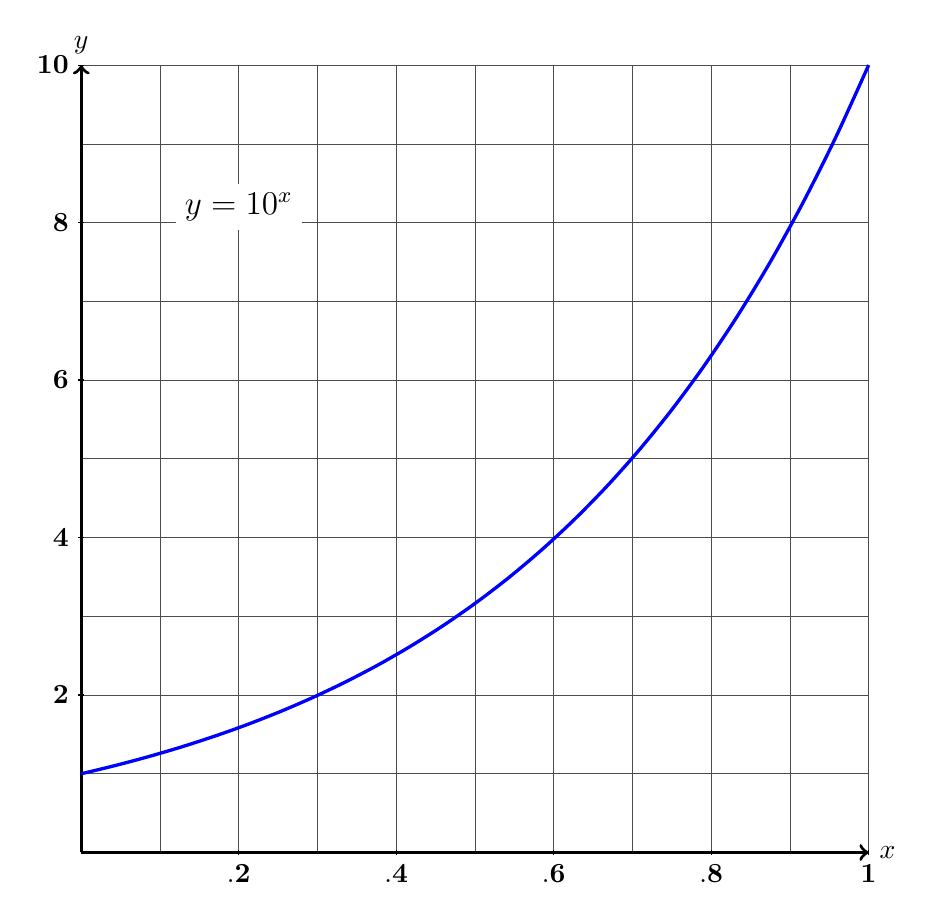
\begin{tikzpicture}
 %grid
  \draw[step=1cm,black!70,very thin] (0,0) grid (10,10);
  %axes
  \draw[very thick,->] (0,0) -- (10,0) node[anchor= west] {\bf{$x$}};
  \draw[very thick,->] (0,0) -- (0,10) node[anchor=south] {\bf{$y$}};
  \foreach \x in {.2,.4,.6,.8,1}
    \draw (10*\x cm,1pt) -- (10*\x cm,-1pt) node[anchor=north] {$\mathbf{\x}$};
  \foreach \y in {2,4,6,8,10}
    \draw (1pt,\y cm) -- (-1pt,\y cm) node[anchor=east] {$\mathbf{\y}$};
   %Function Name
   \node[black,fill=white] at (2,8.2)
   {{\large $y=10^x$}};
   %function
   \draw[scale=1.0,domain=0:10,smooth,variable=\x,blue,very thick] plot (\x,{10^(.1*\x)})
   %Code from previous exam below:
   %\draw[thick,black] plot[domain=0:10] (\x,{10^(.1*\x)})
   ;
 \end{tikzpicture}
\begin{enumerate} 

\item ({\it 1pt}) $10^{1.954}$
\vfill \\ 
\phantom{.} \hfill$ \ $ \ansbox{200}{70} 

\item ({\it 2pts}) $\log(6.310/2.512)$
\vfill \\ 
\phantom{.} \hfill$ \ $ \ansbox{200}{70} 

\item ({\it 3pts}) $\log(\sqrt[5]{200})$
\vfill \\ 
\phantom{.} \hfill$ \ $ \ansbox{200}{70} 
\end{enumerate} 



%%%%%%%%%%% (2)
\item ({\it 2pts}) Solve the following equations. Leave logs in your answer, either base 10 or base 2, but simplify everything else. 
$$2^{2x-3} = 10^{15} $$
\vspace{30pt} \\ \phantom{.} \hfill$ \ x= \ $ \ansbox{200}{70} 

%%%%%%%%%%% (3)
%\newpage
\item ({\it 3pt}) Line A goes through the points $(2,6)$, $(4,4)$. Line B has slope $\frac{2}{3}$ and goes through the point $(6,7)$. 
\begin{enumerate} 
\item ({\it 1pt}) What is the equation of line $A$? Give the answer in the form $y=mx + b$. 
\vspace{80pt} \\ \phantom{.} \hfill$ \ y= \ $ \ansbox{200}{70} 
\item ({\it 1pt}) What is the equation of line $B$? Give the answer in the form $y=mx + b$. 
\vspace{80pt} \\ \phantom{.} \hfill$ \ y= \ $ \ansbox{200}{70} 
\item ({\it 1pt}) What are the coordinates of the point where the lines $y=3+x$ and $y=9-x$ intersect? 
\vspace{80pt} \\ \phantom{.} \hfill$ \ (x,y)= \ $ \ansbox{200}{70} 
\end{enumerate}


%%%%%%%%%%% (4)
\item ({\it 3 pts}) 
The distance traveled by a race car $t$ seconds after leaving the starting line is modeled by $f(t) =t^2$ meters. 
\begin{enumerate}
\item ({\it 1 pt})
Find the average speed of a race car over the time period from 2 seconds to $2.1$ seconds. 
\vfill\\
\phantom{.} \hfill\ansbox{120}{70} \ $m/s$ \\
\item ({\it 2 pts})
Find the average speed of a race car over the time period from 2 seconds to $2+h$ seconds for a small time interval $h$. 
\vfill\\
\vfill\\
\phantom{.} \hfill\ansbox{200}{100} \ $m/s$ 





\end{enumerate}



%%%%%%%%%%% (5)
\newpage
\item ({\it 2pts}) Initially can A contains 6 liters of red paint and can B contains 12 liters of blue paint. I pour 1/2 of the red paint into can B. After mixing the paint in can B, I pour 1/2 of the paint in can B into can A. \\ \\
How many liters of blue paint are now in can A? 
\vfill \\ \phantom{.} \hfill \ansbox{200}{70} L
 
%%%%%%%%%%% (6)
\item ({\it 2 pts}) Back in 2013, an enterprising 34A student observed that many students forgot to bring 3x5 note cards with them to campus. She had plenty of packages of note cards lying around that she needed to get rid of by the end of the year and she decided to sell them to students on campus. If she charged 10 cents a card, she would sell 500 cards and make \$50 (why?). But for each cent she increased the price, the number of cards she sold would decrease by 10. 
\begin{enumerate}
\item ({\it 1 pt}) If she had picked a price of $10 + x$ cents for each card, how many cards will she sell? 
\vfill \\ \phantom{.} \hfill  \ansbox{150}{70} cards
\item ({\it 1 pts}) What is the total amount of money (in cents) she would have received from selling cards for $10 + x$ cents each. Please simplify your answer, which should of course be in terms of $x$. \\ 
\vfill
\phantom{.} \hfill 
\ansbox{200}{70} \ {\Large \textcent}
\end{enumerate}



%%%%%%%%%%% (7)
\newpage

\item ({\it 2 points}) Compute the following sum (don't just list the terms in it). 
$$\sum_{n=3}^5 \frac{n(n+1)}{2}$$
\\ \phantom{.} \hfill\ansbox{140}{70} 
\vfill \\  

%%%%%%%%%%% (8)
%\newpage
\item ({\it 2 points}) What are the following limits? 
\begin{enumerate} 
\item ({\it 1pt}) {\large $\underset{h \rightarrow 0}{\lim} \ \ $} {\Large $\frac{7+4h-7}{h}$} \\ \\ \phantom{.} \hfill\ansbox{140}{70} 
\vfill \\  
\item ({\it 1pt}) {\large $\underset{h \rightarrow 0}{\lim}$} \ \ {\large $\frac{50 + 20h + 2h^2 - 50}{h}$} 
\vfill \\ 
\phantom{.} \hfill\ansbox{140}{70} \\ \\  
\end{enumerate}

\newpage
%%%%%%%%%%% (9)
\item ({\it 2pts}) A square garden consists of a semicircular pond and the rest is a lawn. The length of each side of the square garden is $\ell$. If the area of the square is 1,600 $m^2$, then find the area of the lawn.  
\\
{\includegraphics[width=4in]{Midterm_2_Pond_Screenshot.png} }
\vfill \\ 
\phantom{.} \hfill lawn area$ \ = \ $ \ansbox{200}{70}$\ m^2$ 
















\end{enumerate}



\end{document}

